\documentclass{beamer}

\mode<presentation>
{
  \usetheme{default}
  \usecolortheme{default}
  \usefonttheme{default}
  \setbeamertemplate{navigation symbols}{}
  \setbeamertemplate{caption}[numbered]
  \setbeamertemplate{footline}[page number]
  \setbeamercolor{frametitle}{fg=white}
  \setbeamercolor{footline}{fg=black}
} 

\usepackage[english]{babel}
\usepackage[utf8x]{inputenc}
\usepackage{tikz}
\usepackage{listings}
\usepackage{courier}
\usepackage{array}
\usepackage{bold-extra}
\usepackage{minted}

\xdefinecolor{darkblue}{rgb}{0.1,0.1,0.7}
\xdefinecolor{darkgreen}{rgb}{0,0.5,0}
\xdefinecolor{darkgrey}{rgb}{0.35,0.35,0.35}
\xdefinecolor{darkorange}{rgb}{0.8,0.5,0}
\xdefinecolor{darkred}{rgb}{0.7,0,0}
\xdefinecolor{dianablue}{rgb}{0.18,0.24,0.31}
\definecolor{commentgreen}{rgb}{0,0.6,0}
\definecolor{stringmauve}{rgb}{0.58,0,0.82}

\lstset{ %
  backgroundcolor=\color{white},      % choose the background color
  basicstyle=\ttfamily\small,         % size of fonts used for the code
  breaklines=true,                    % automatic line breaking only at whitespace
  captionpos=b,                       % sets the caption-position to bottom
  commentstyle=\color{commentgreen},  % comment style
  escapeinside={\%*}{*)},             % if you want to add LaTeX within your code
  keywordstyle=\color{blue},          % keyword style
  stringstyle=\color{stringmauve},    % string literal style
  showstringspaces=false,
  showlines=true
}

\lstdefinelanguage{scala}{
  morekeywords={abstract,case,catch,class,def,%
    do,else,extends,false,final,finally,%
    for,if,implicit,import,match,mixin,%
    new,null,object,override,package,%
    private,protected,requires,return,sealed,%
    super,this,throw,trait,true,try,%
    type,val,var,while,with,yield},
  otherkeywords={=>,<-,<\%,<:,>:,\#,@},
  sensitive=true,
  morecomment=[l]{//},
  morecomment=[n]{/*}{*/},
  morestring=[b]",
  morestring=[b]',
  morestring=[b]"""
}

\title[2017-05-03-future-trends]{Lowering boundaries between \\ data analysis ecosystems}
\author{Jim Pivarski}
\institute{Princeton University -- DIANA Project}
\date{May 3, 2017}

\begin{document}

\logo{\pgfputat{\pgfxy(0.11, 8)}{\pgfbox[right,base]{\tikz{\filldraw[fill=dianablue, draw=none] (0 cm, 0 cm) rectangle (50 cm, 1 cm);}}}\pgfputat{\pgfxy(0.11, -0.6)}{\pgfbox[right,base]{\tikz{\filldraw[fill=dianablue, draw=none] (0 cm, 0 cm) rectangle (50 cm, 1 cm);}
\includegraphics[height=0.99 cm]{diana-hep-logo.png}\tikz{\filldraw[fill=dianablue, draw=none] (0 cm, 0 cm) rectangle (4.9 cm, 1 cm);}}}}

\begin{frame}
  \titlepage
\end{frame}

\logo{\pgfputat{\pgfxy(0.11, 8)}{\pgfbox[right,base]{\tikz{\filldraw[fill=dianablue, draw=none] (0 cm, 0 cm) rectangle (50 cm, 1 cm);}
\includegraphics[height=1 cm]{diana-hep-logo.png}}}}

% Uncomment these lines for an automatically generated outline.
%\begin{frame}{Outline}
%  \tableofcontents
%\end{frame}

%%%%%%%%%%%%%%%%%%%%%%%%%%%%%%%%%%%%%%%%%%%%%%%%%%%%%%%

\begin{frame}{Data analysis ecosystems}
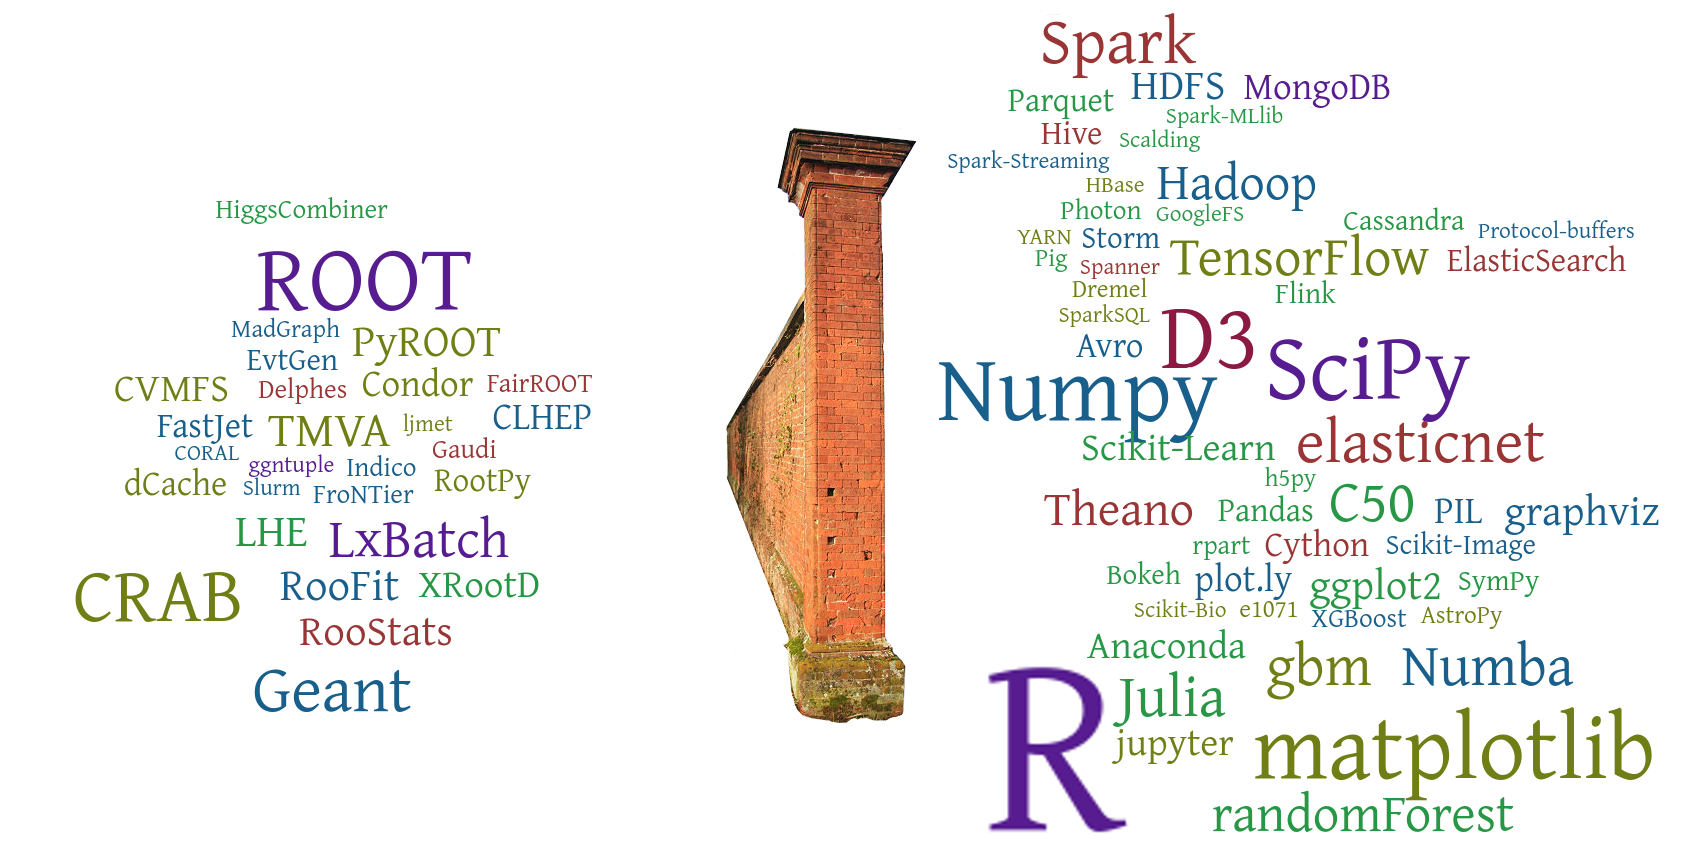
\includegraphics[width=\linewidth]{separation.png}
\end{frame}

\begin{frame}{}
\begin{center}
\large \textcolor{darkblue}{Physicists developed their own software for a good reason:}

\textcolor{darkblue}{no one else was tackling such large problems.}
\end{center}
\end{frame}

\begin{frame}{Not so today\ldots}
\vspace{0.5 cm}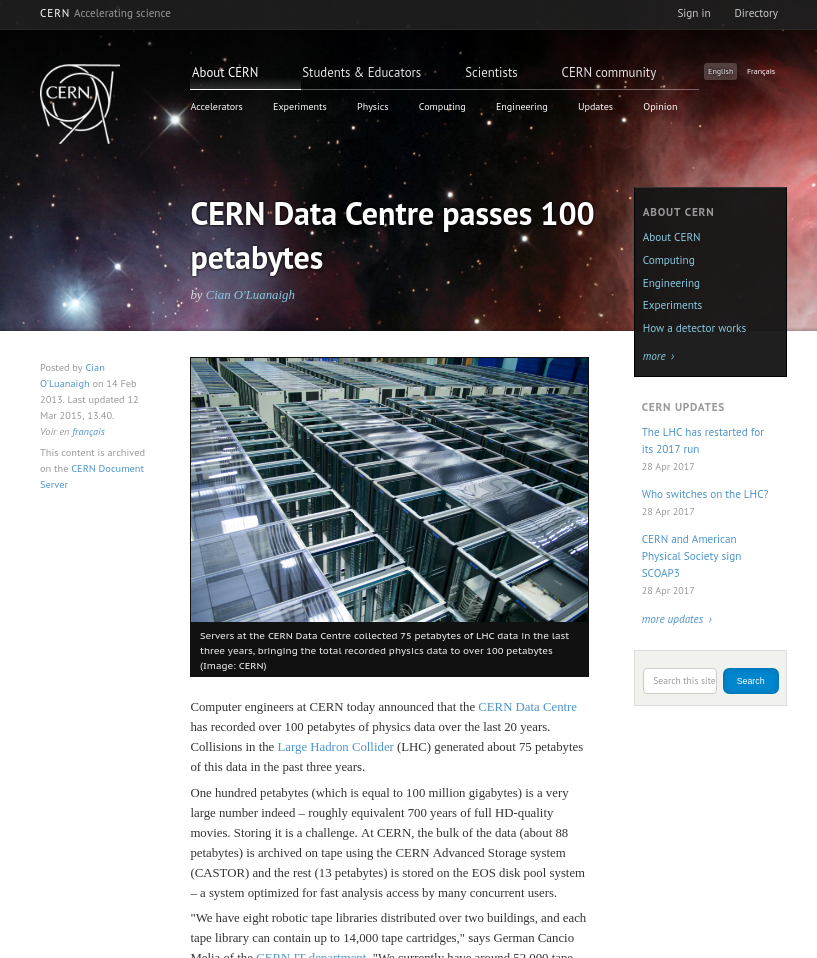
\includegraphics[width=0.75\linewidth]{cern_petabytes.png}

\vspace{-6.4 cm}\only<2>{\hfill 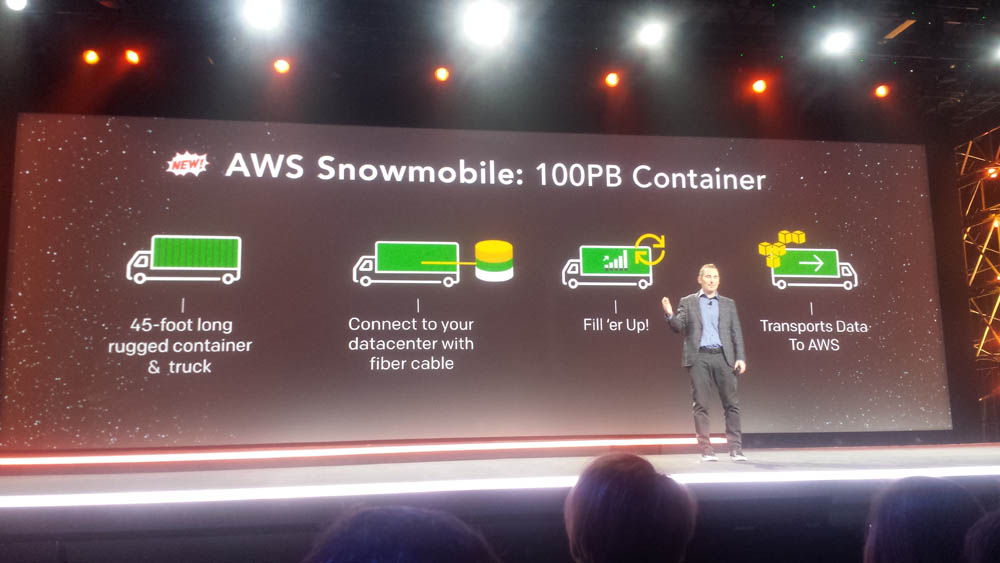
\includegraphics[width=0.75\linewidth]{aws-snowmobile.jpg}}\vspace{6.4 cm}
\end{frame}

\begin{frame}{Case in point: ROOT and Spark}
\vfill
\textcolor{darkblue}{Relative rate of web searches (Google Trends):}

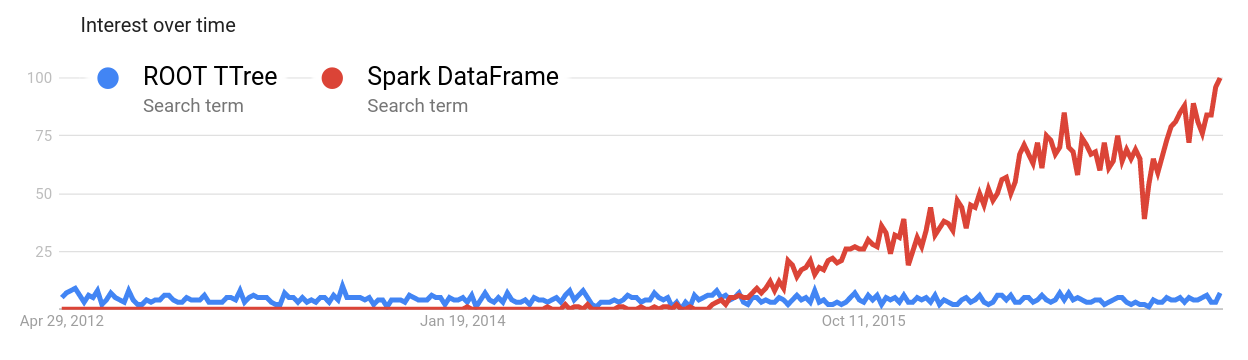
\includegraphics[width=\linewidth]{root-spark-google-trends.png}

\vfill
\textcolor{darkblue}{Question-and-answer sites:}
\begin{itemize}
\item RootTalk: 14,399 threads in 1997--2012 (15 years)
\item StackOverflow questions tagged \#spark: 26,155 in the 3.3 years it has existed.
\end{itemize}

\vfill
\textcolor{darkblue}{More users to talk to; more developers adding features/fixing bugs.}
\end{frame}

\begin{frame}{Building bridges: low effort-to-reward}
\vspace{0.5 cm}
\begin{center}
\hspace{1 cm}\only<1>{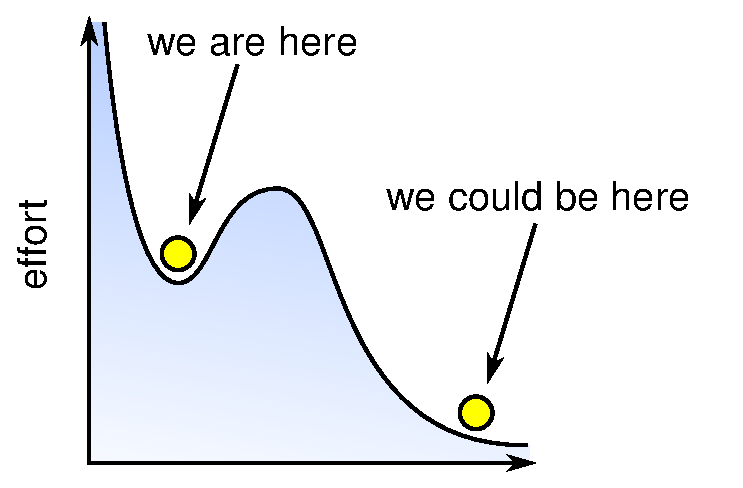
\includegraphics[width=0.75\linewidth]{effort0.pdf}}\only<2>{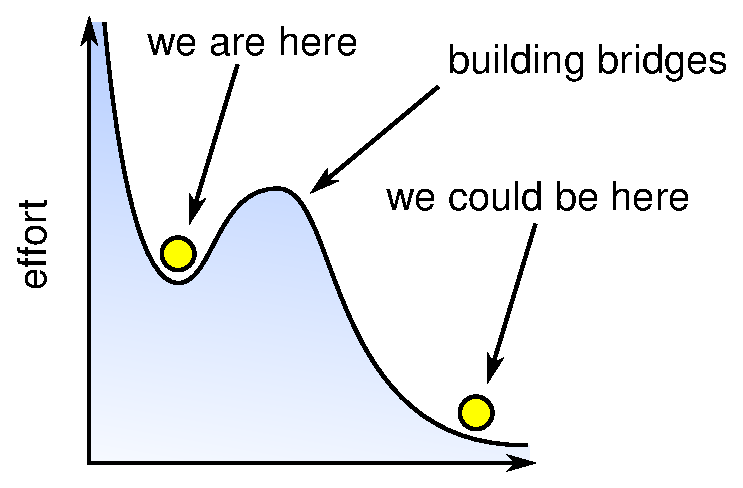
\includegraphics[width=0.75\linewidth]{effort.pdf}}
\end{center}
\end{frame}

\begin{frame}{Who am I?}
\begin{columns}[t]
\column{0.55\linewidth}
\begin{columns}
\column{0.4\linewidth}
Jim Pivarski
\column{0.2\linewidth}
\hspace{-1.3 cm}
\includegraphics[width=\linewidth]{faces/jim_pivarski.png}
\end{columns}

\begin{itemize}
\item 5 years CLEO (9 GeV $e^+e^-$)
\item 5 years CMS (7 TeV $pp$)
\item \only<1>{5 years Open Data Group}\only<2>{\mbox{\textcolor{darkblue}{5 years Open Data Group \hspace{0.4 cm}$\longrightarrow$\hspace{-3 cm}}}}
\item 1+ years Project DIANA-HEP
\end{itemize}

\column{0.5\linewidth}
\uncover<2>{\textcolor{darkblue}{
hyperspectral imagery \\
automobile traffic \\
network security \\
Twitter sentiment \\
Google n-grams \\
DNA sequence analysis \\
credit card fraud detection
}}

\uncover<2>{\Large\textcolor{darkblue}{ and ``Big Data'' tools}}
\end{columns}
\end{frame}

\begin{frame}{}

\only<1>{\mbox{\hspace{-1 cm}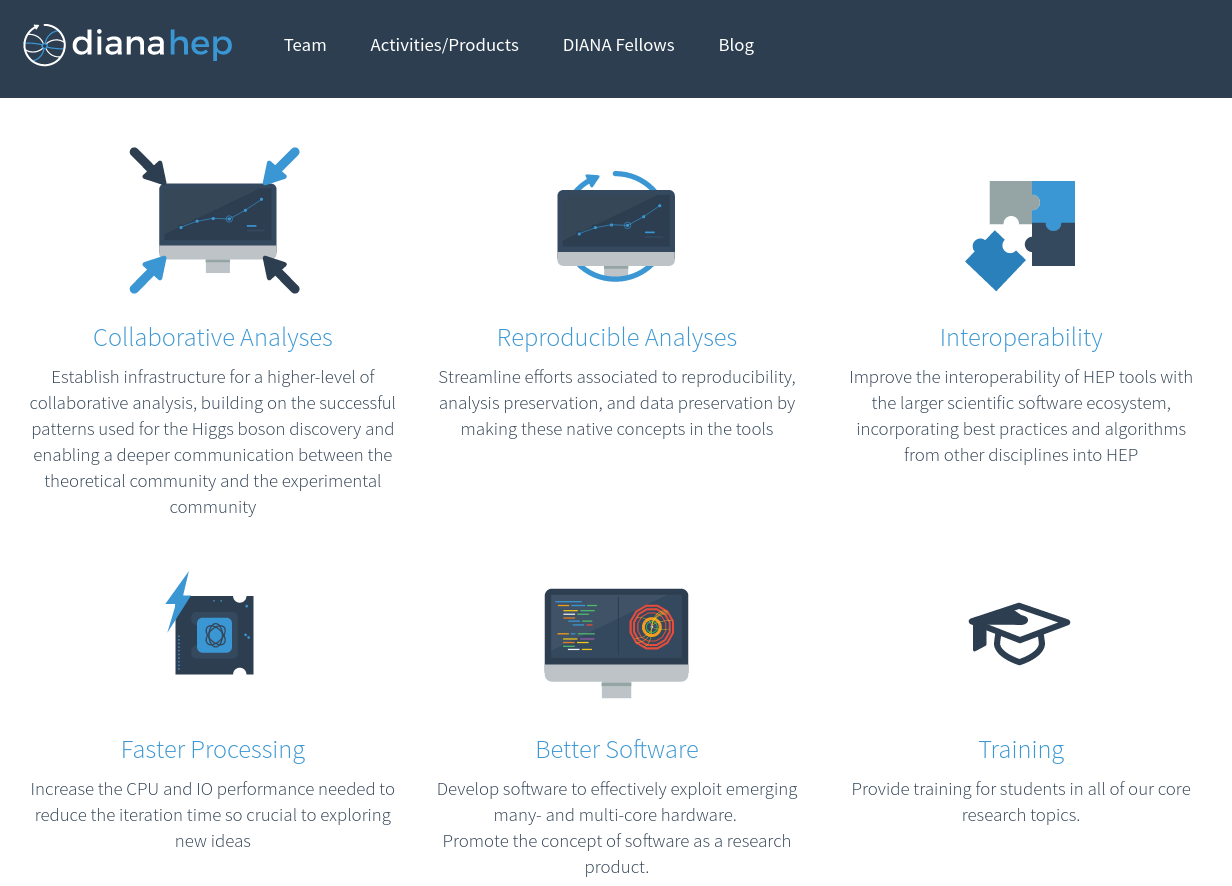
\includegraphics[width=1.2\linewidth]{diana-hep.png}}}
\only<2>{\mbox{\hspace{-1 cm}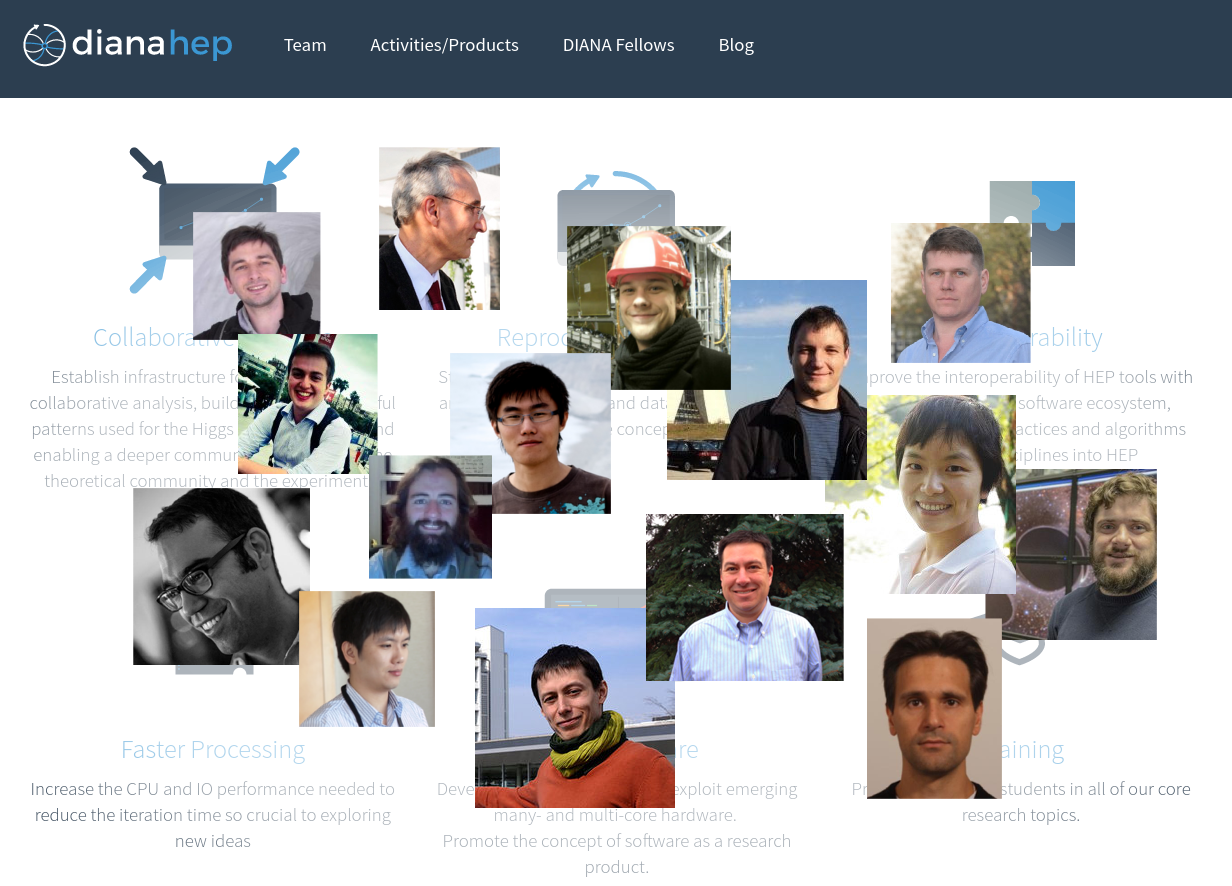
\includegraphics[width=1.2\linewidth]{diana-hep2.png}}}

\end{frame}

\begin{frame}{Outline of this talk}
\Large
\begin{description}\setlength{\itemsep}{0.5 cm}
\item[Data plumbing:] a CMS analysis in Apache Spark
\item[Histogrammar:] HEP-like tools in a functional world
\item[Femtocode:] the ``query system'' concept in HEP
\end{description}
\end{frame}

\begin{frame}{Apache Spark}
\vspace{0.5 cm}
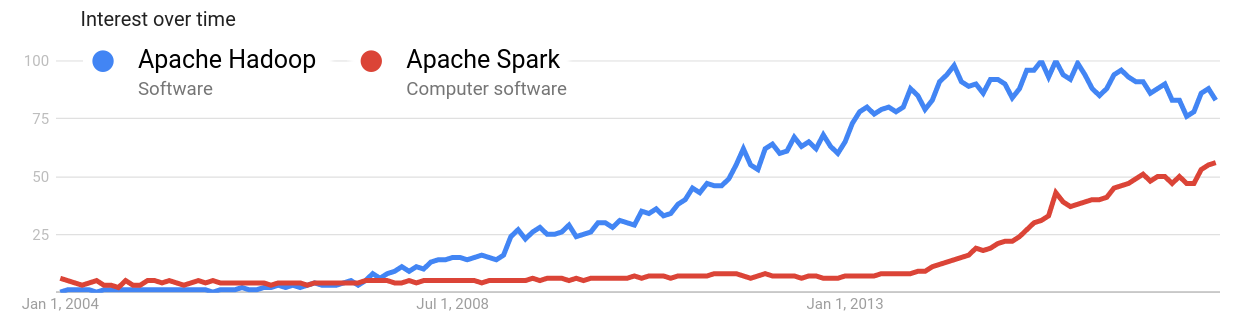
\includegraphics[width=\linewidth]{hadoop-versus-spark.png}

\vfill

\includegraphics[width=0.25\linewidth]{spark.png}

\begin{itemize}
\item Like Hadoop in that it implements map-reduce, but these are just two out of many functionals.
\item Not a competitor: can run on a Hadoop cluster.
\item Primary interface is a console: each command does a distributed job and returns a result.
\item User controls in-memory cache on the cluster, effectively getting an $\mathcal{O}(\mbox{TB})$ working space in RAM.
\end{itemize}
\end{frame}

\begin{frame}{CMS analysis on Spark}
\vfill
\begin{itemize}
\item Oliver Gutsche, Matteo Cremonesi, Cristina Su\'arez (Fermilab) wanted to try their CMS dark matter search on Spark.
\item My first project with DIANA-HEP: I joined to plow through technical issues before the analysts hit them.

\vfill
\begin{center}
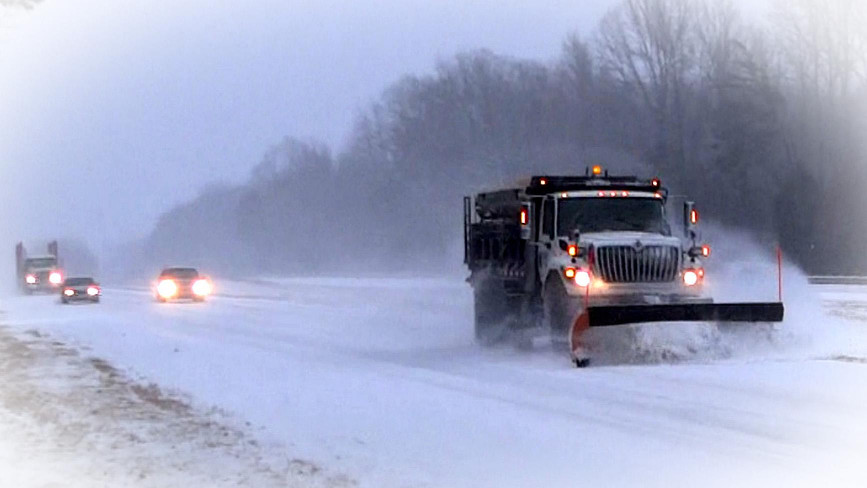
\includegraphics[width=0.75\linewidth]{snowplow.jpg}
\end{center}
\end{itemize}
\end{frame}

\begin{frame}{Problems!}
\Large

\begin{enumerate}\setlength{\itemsep}{0.5 cm}
\item Need a Spark cluster.

\item Spark, like most ``Big Data'' tools, runs on the Java Virtual Machine (JVM), not C++, and doesn't recognize our ROOT data format.

\item HEP analysis tools like histograms don't have the right API to fit Spark's functional interface.

\end{enumerate}
\end{frame}

\begin{frame}{\#1. Need a Spark cluster}
Several other groups are interested in this and were willing to share resources in exchange for having us test their system.

\begin{itemize}
\item Alexey Svyatkovskiy (Princeton) was active in the group, helping us use the Princeton BigData cluster.
\item Saba Sehrish and Jim Kowalkowski (Fermilab) modified the analysis for NERSC.
\item Maria Girone, Luca Canali, Kacper Surdy (CERN), and Vaggelis Motesnitsalis (Intel) are now setting up a Data Reduction Facility at CERN as an OpenLab project.
\end{itemize}
\end{frame}

\begin{frame}{\#2. Getting data from ROOT files into JVM}
\vspace{0.3 cm}
\small

\textcolor{darkblue}{\normalsize A run-down of the attempted solutions\ldots}
\begin{enumerate}
\item \textcolor{darkblue}{Java Native Interface (JNI)} \\ No! This ought to be the right solution, but Java \\ and ROOT are both large, complex applications \\ with their own memory management: couldn't keep \\ them from interfering (segmentation faults).

\vspace{-2.2 cm}
\hfill 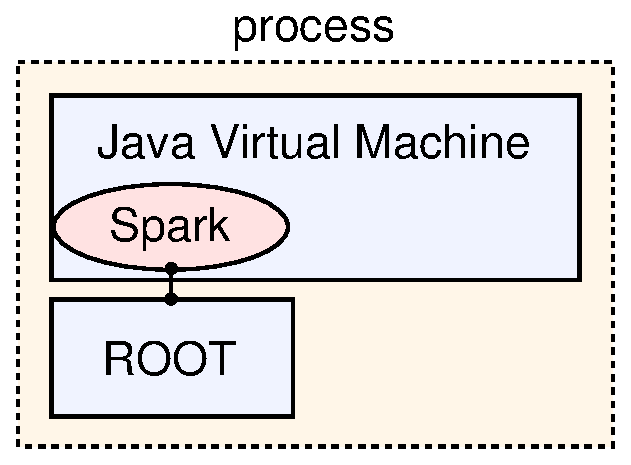
\includegraphics[height=1.65 cm]{root-spark.pdf}

\vspace{0.5 cm}
\item \textcolor{darkblue}{\normalsize Python as glue: PyROOT and PySpark in the same process}

\hfill 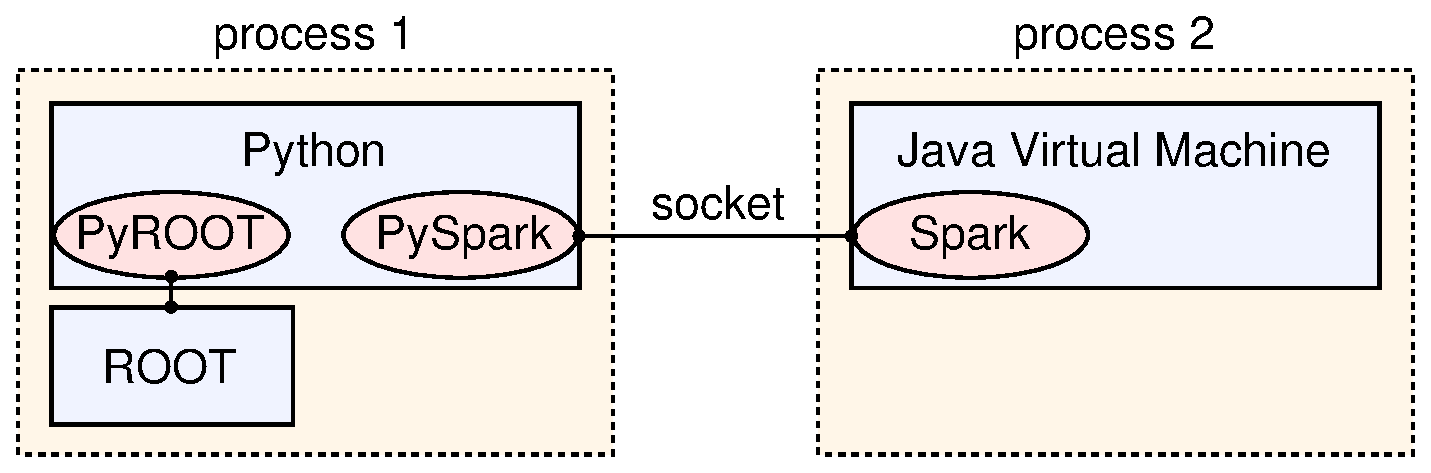
\includegraphics[height=1.65 cm]{pyroot-pyspark.pdf}

\vspace{-1.8 cm}
PySpark is a low-performance \\ solution: all data must be passed \\ over a text-based socket and \\ interpreted by Python.

\item \textcolor{darkblue}{\normalsize Convert to a Spark-friendly format, like Apache Avro}

We used this for a year. Efficient after conversion, but that conversion step is awkward. Avro's C library is difficult to deploy.

\item \textcolor{darkblue}{\normalsize Use pure Java code to read ROOT files}

What we do now. It's worth it.

\end{enumerate}
\end{frame}

\begin{frame}{}

\only<1>{{\mbox{\hspace{-1 cm}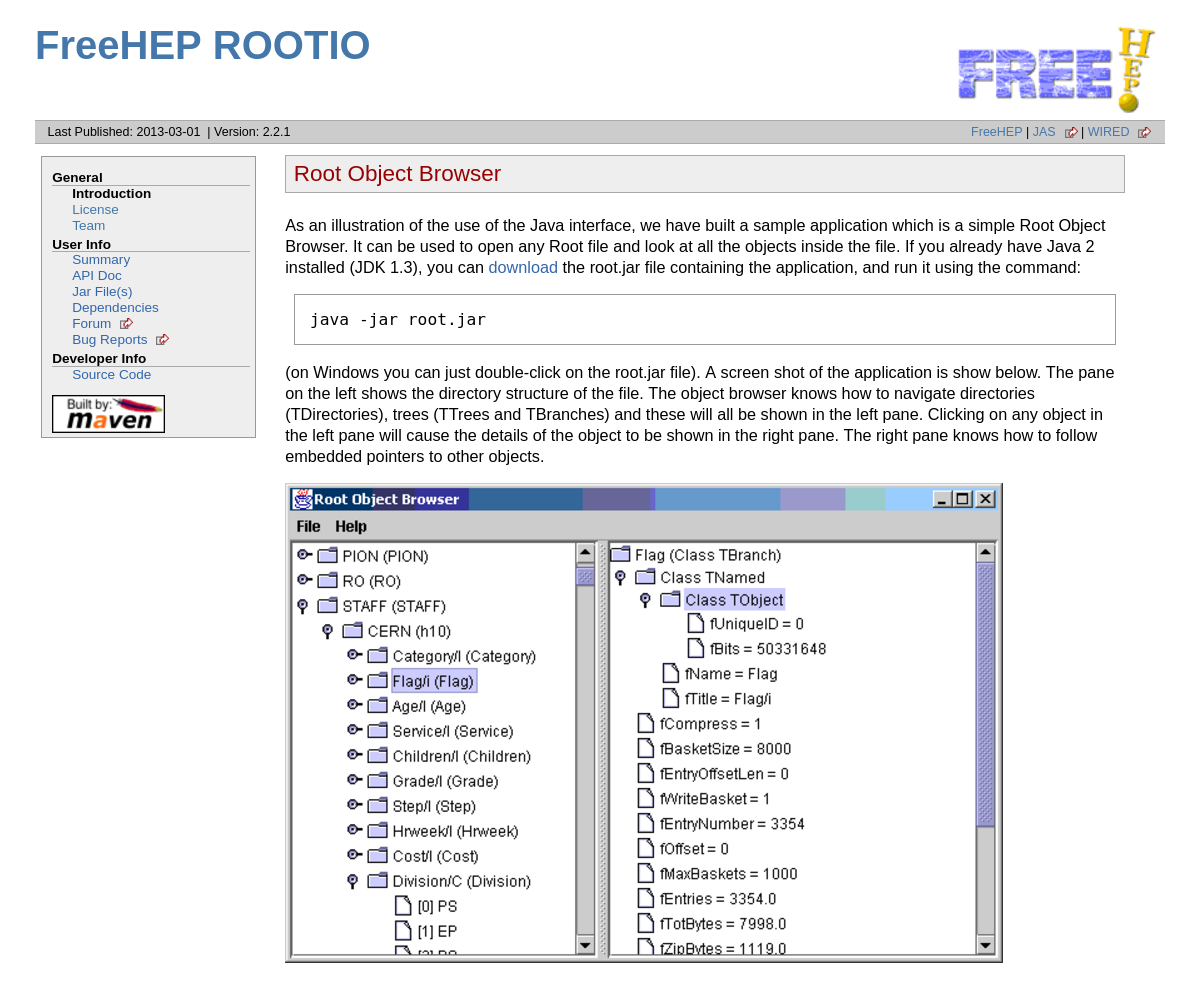
\includegraphics[width=1.2\linewidth]{rootio-screenshot.png}}}}
\only<2->{{\mbox{\hspace{-1 cm}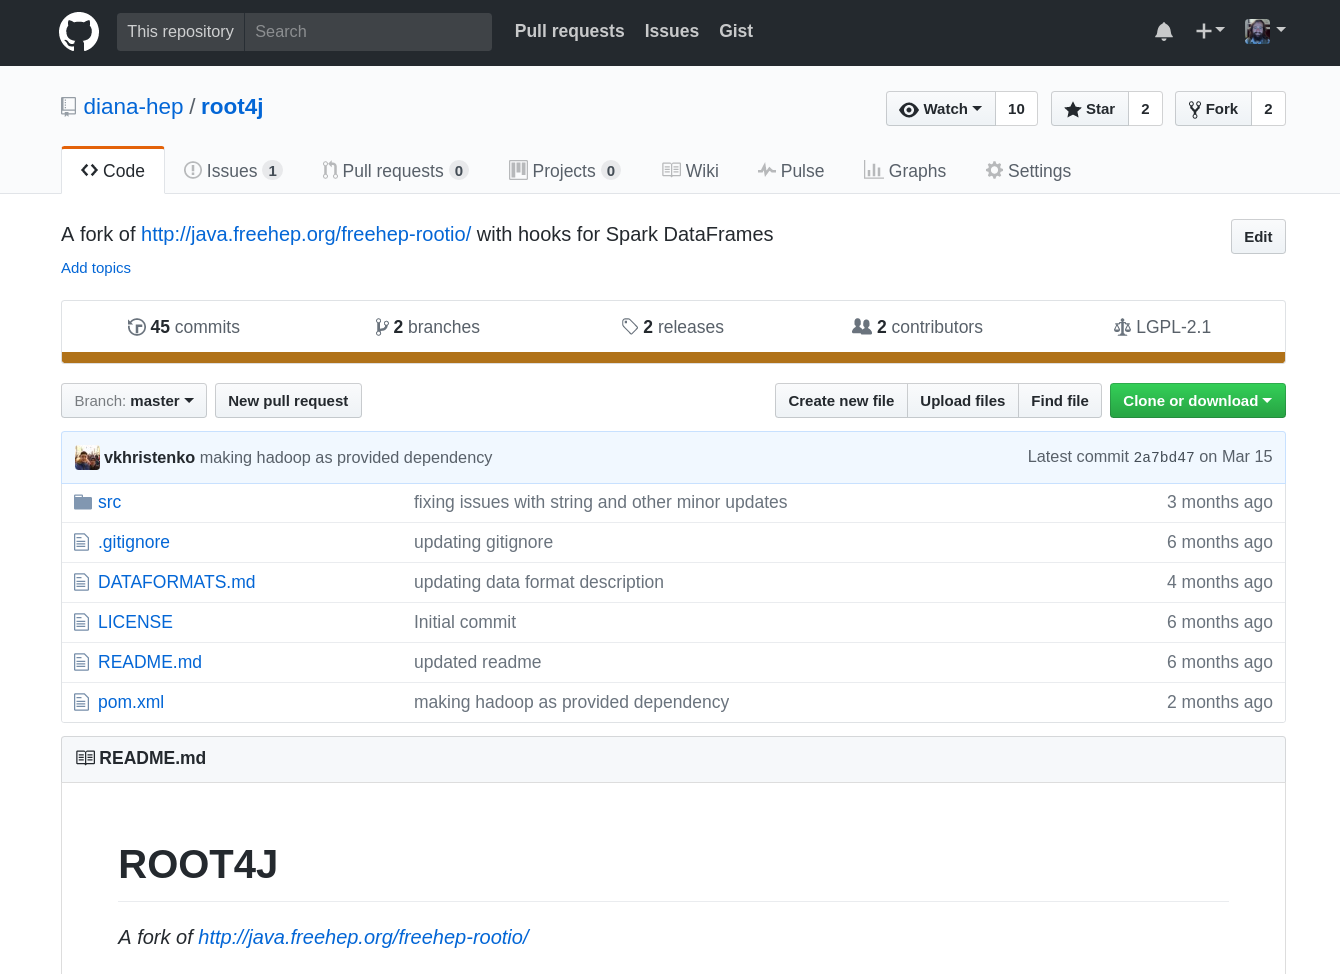
\includegraphics[width=1.2\linewidth]{root4j.png}}}}

\begin{onlyenv}<3>
\vspace{-3.5 cm}\hfill\begin{minipage}{3 cm}
\begin{center}
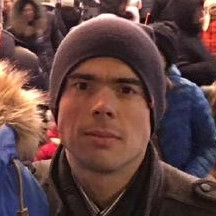
\includegraphics[width=2 cm]{viktor.jpg}

Viktor Khristenko

{\small University of Iowa}
\end{center}
\end{minipage}\hspace{1 cm}\vspace{3.5 cm}
\end{onlyenv}

\end{frame}


\end{document}
